\section{From separating filtrations to finite chains}\label{sec:chains}

Fix the dimension $n$ and radii chosen in Section~\ref{sec:metric}.
For each $\epsilon>0$, use the filtration supplied by
Proposition~\ref{prop:zero-strata}. We will turn it into an
$H$-equivariant chain map
\[
 F^\epsilon:C_*(K)\longrightarrow E_*
\]
that is equivariantly chain homotopic to inclusion. Its evaluation by
a fixed invariant cocycle will tend to zero. These two properties
prove Theorem~\ref{thm:sparse}. Throughout this section $n$ remains
fixed while $\epsilon$ tends to zero.

\subsection{Component averages and their finite support}

For a fixed parameter $x$, take the barycentric subdivision of the
final triangulation $T_0(x)$. Its vertices are the barycenters $b_F$
of nonempty simplices $F$ of $T_0(x)$. Define
\[
 \ell(F)=\min\{i:b_F\in Z_i(x)\},
 \qquad Z_{-1}(x)=\varnothing.
\]
All $Z_i(x)$ are subcomplexes of $T_0(x)$, so $b_F\in Z_i(x)$
is equivalent to $F\subseteq Z_i(x)$. Let $U_F$ be the connected
component of $Z_{\ell(F)}(x)\setminus Z_{\ell(F)-1}(x)$ containing
$b_F$. For any such component $U$, set
\begin{equation}\label{eq:component-average}
 J_U=\bigcup_{p\in U}\supp p,
 \qquad
 u_U=\frac{1}{|J_U|}\sum_{v\in J_U}\delta_v.
\end{equation}
The next lemma proves that $J_U$ is finite and controls these
labels as $x$ varies.  The intended image of an oriented barycentric
simplex is
\begin{equation}\label{eq:exterior-replacement}
 [b_{F_0},\ldots,b_{F_j}]
 \longmapsto u_{U_{F_0}}\wedge\cdots\wedge u_{U_{F_j}}\in E_j.
\end{equation}

This choice uses the separating filtration in a specific way.
If nested faces $F\subset F'$ have the same level $i$, the segment
joining their barycenters lies in $Z_i\setminus Z_{i-1}$.
Except at its endpoint $b_F$, it lies in the relative interior
of $F'$, which the subcomplex $Z_{i-1}$ misses; the endpoint also
avoids $Z_{i-1}$ by its level.  The two barycenters therefore receive
the same component vector, making any exterior term containing
both zero.  Along a complete flag $F_0\subset\cdots\subset F_n$,
with $\dim F_i=i$, the levels are nondecreasing: if
$F\subset F'\subseteq Z_i$, then $F\subseteq Z_i$.
A nonzero image must consequently use all levels $0,1,\ldots,n$,
beginning at a point of $Z_0$.  We will bound the number of these
flags after establishing that the labels define finite chains.

\begin{lemma}\label{lem:finite-component-labels}
For every original simplex $\kappa$ of $K$, there is a finite set
$W_\kappa\subseteq Y$, independent of $\epsilon$ and $x$, such that
$J_{U_F}\subseteq W_\kappa$ whenever $b_F\in\kappa$. The triangulation
over $\kappa$, together with all its assigned vectors $u_{U_F}$,
is locally constant in $x$. These assignments are equivariant.
\end{lemma}

\begin{proof}
Each component of $Z_i(x)\setminus Z_{i-1}(x)$ has
$\rho$-diameter at most $2R$. For $i=0$ the components are
singletons, since $Z_0(x)$ is a locally finite zero-dimensional
subcomplex. If $b_F\in\kappa$ and $p\in U_F$, the support-distance
bound from Lemma~\ref{lem:proper} gives
\[
 \min d_Y(\supp b_F,\supp p)
 \leq\sqrt n\,\rho(b_F,p)\leq 2R\sqrt n.
\]
Choose an original top simplex containing $p$. Its $n+1$ vertices
span a connected graph, so every vertex in $\supp p$ is within
graph distance $n$ of the vertex furnished by this inequality.
Consequently we may take
\[
 W_\kappa=
 \left\{v\in Y:
 d_Y\bigl(v,V(\kappa)\bigr)
 \leq\left\lceil 2R\sqrt n+n\right\rceil\right\}.
\]
The bounded degree of $Y$ makes this set finite. Notice that the
support of $p$ need not itself span a connected graph; we used
the containing top simplex.

Let $K[W_\kappa]$ be the finite subcomplex consisting of the simplices
whose vertices belong to $W_\kappa$. The whole component $U_F$
lies in its realization. It follows that $U_F$ is exactly the
component containing $b_F$ in
\[
 \bigl(Z_{\ell(F)}(x)\setminus Z_{\ell(F)-1}(x)\bigr)
 \cap |K[W_\kappa]|.
\]
Indeed $U_F$ is a connected subset of this restriction, and every
connected subset of the restriction containing $b_F$ also lies in
the original component. Thus restricting to this finite subcomplex
does not cut off a part of the component needed to compute $J_{U_F}$.

There are finitely many original simplices in $K[W_\kappa]$.
A common refinement of their finite clopen parameter partitions
makes all their triangulation and filtration data constant.
On each resulting piece the components and their sets of support
vertices are constant as well. This proves local constancy of
the assignments over $\kappa$. Finally,
$J_{hU}=hJ_U$, and hence $u_{hU}=h u_U$, proving equivariance.
\end{proof}

Subdivide each oriented original simplex into its fundamental
subdivision chain and apply the exterior assignment
\eqref{eq:exterior-replacement} to every term. This defines a map
$f_x:C_*(K)\to E_*$. Both operations commute
with the augmented boundary. For subdivision, interior facets
cancel in pairs and the boundary facets give the compatible
subdivision on each original face. For the second operation,
each assigned vector has coefficient sum one, so contraction
with the coefficient-sum functional gives
\[
 \partial(u_0\wedge\cdots\wedge u_j)
 =\sum_{i=0}^j(-1)^i
 u_0\wedge\cdots\wedge\widehat{u_i}\wedge\cdots\wedge u_j.
\]
Thus $f_x$ is an augmented chain map.

By Lemma~\ref{lem:finite-component-labels}, its value on any
original simplex is constant on a finite clopen partition and
is supported in a fixed finite exterior space. We may therefore
define
\begin{equation}\label{eq:averaged-chain-map}
 F^\epsilon(c)=\int_X f_x(c)\,d\mu(x).
\end{equation}
This integral is an actual finite chain: for every $c$ it is a
finite linear combination of finitely many chain values.
It commutes with the augmented boundary. Moreover,
$f_{hx}(hc)=h f_x(c)$, so invariance of $\mu$ shows that
$F^\epsilon$ is $H$-equivariant.

\subsection{Counting the surviving flags}

We now bound the evaluation of $f_x$ on a top simplex. The number
of subdivision simplices may depend on $\epsilon$; the following
bound depends instead on the number of zero-stratum points.
The component-labeling and flag-counting method is modeled on
Alpert \cite[Lemmas 4 and 10]{Alpert2025}; the carrier argument below
supplies the bound without a manifold hypothesis.

\begin{lemma}\label{lem:surviving-flags}
For every original top simplex $\sigma$ and every $x$, at most
\[
 2^n\#\bigl(Z_0(x)\cap\sigma\bigr)
\]
terms in its fundamental barycentric subdivision chain have
nonzero images under the exterior replacement map.
\end{lemma}

\begin{proof}
Suppress $x$. Such a term corresponds to a complete flag
\[
 F_0\subset F_1\subset\cdots\subset F_n,
 \qquad \dim F_i=i,
\]
in the restriction of $T_0$ to $\sigma$. As shown when defining
\eqref{eq:exterior-replacement}, a nonzero term has levels exactly
$0,1,\ldots,n$. In particular $F_0=\{z\}$ for a point
$z\in Z_0\cap\sigma$ and $F_i\subseteq Z_i$ for every $i$.

By Lemma~\ref{lem:carrier}, $z$ lies in the relative interior of
a unique $i$-simplex $S_i$ of $T_i$ contained in $Z_i$. To see why
this carrier controls the final refinement, let $F_i$ occur in a
surviving flag through $z$. The $T_i$-carrier of a relative-interior
point of $F_i$ contains $F_i$ by refinement and belongs to $Z_i$,
because $Z_i$ is a subcomplex. That carrier has dimension at least
$i$, since it contains $F_i$, and at most $i$, since $\dim Z_i\leq i$.
It contains $z$, so it equals $S_i$. Hence $F_i\subseteq S_i$.

For a fixed preceding face $F_{i-1}$, the possible $F_i$ are thus
full-dimensional simplices in a triangulation of the single affine
$i$-simplex $S_i$, having $F_{i-1}$ as a facet. There is at most one
on either side of the affine hyperplane spanned by that facet.
Otherwise two simplices on the same side would have intersecting
relative interiors near an interior point of the facet. There
are therefore at most two choices at each stage and at most $2^n$
surviving flags through $z$. Summing over $z$ proves the assertion.
This argument concerns one carrier simplex at a time and uses no
manifold assumption on $K$ or on the strata.
\end{proof}

Figure~\ref{fig:flags} illustrates the two choices at each of the two
stages when $n=2$.

\begin{figure}[htbp]
\centering
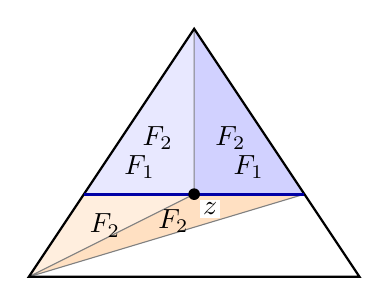
\begin{tikzpicture}[scale=1.05]
 \coordinate (A) at (-2,0);
 \coordinate (B) at (2,0);
 \coordinate (C) at (0,3);
 \coordinate (L) at (-1.3333,1);
 \coordinate (R) at (1.3333,1);
 \coordinate (z) at (0,1);
 \fill[blue!9] (L)--(z)--(C)--cycle;
 \fill[blue!18] (z)--(R)--(C)--cycle;
 \fill[orange!13] (L)--(z)--(A)--cycle;
 \fill[orange!24] (z)--(R)--(A)--cycle;
 \draw[thin,gray] (z)--(A) (A)--(R) (z)--(C);
 \draw[thick] (A)--(B)--(C)--cycle;
 \draw[very thick,blue!65!black] (L)--(R);
 \fill (z) circle (2pt) node[below right=2pt,fill=white,inner sep=1pt] {$z$};
 \node at (-0.44,1.68) {$F_2$};
 \node at (0.44,1.68) {$F_2$};
 \node at (-1.08,0.62) {$F_2$};
 \node at (-0.25,0.67) {$F_2$};
 \node[above=2pt] at (-0.66,1) {$F_1$};
 \node[above=2pt] at (0.66,1) {$F_1$};
\end{tikzpicture}
\caption{The flag count in dimension two. The point $z\in Z_0$ has
two possible incident edges $F_1$ along its one-dimensional carrier.
Each edge has at most two incident triangles $F_2$ inside the original
two-dimensional carrier. The four shaded triangles give the four possible
flags through $z$ in this example. The unshaded triangle has no
one-dimensional-stratum edge through $z$.}
\label{fig:flags}
\end{figure}

Let $\psi:E_n\to\C$ be the invariant cocycle in
Theorem~\ref{thm:sparse}. For an original top simplex $\sigma$, put
\[
 M_\sigma=
 \max_{v_0,\ldots,v_n\in W_\sigma}
 \left|\psi(\delta_{v_0}\wedge\cdots\wedge\delta_{v_n})\right|.
\]
This is finite, even though $\psi$ need not be bounded on all
basis simplices of the infinite vertex set. Every vector in
\eqref{eq:component-average} is a nonnegative convex combination
of vertices in $W_\sigma$. Multilinearity therefore bounds the
evaluation of each surviving term by $M_\sigma$. The preceding
lemma and Proposition~\ref{prop:zero-strata} give
\begin{align}
 \left|\psi\bigl(F^\epsilon(\sigma)\bigr)\right|
 &\leq 2^n M_\sigma
 \int_X\#\bigl(Z_0(x)\cap\sigma\bigr)\,d\mu(x)
 \notag\\
 &\leq 2^n M_\sigma C_\sigma\epsilon
 \longrightarrow 0.\label{eq:small-chain-evaluation}
\end{align}
All constants here are independent of $\epsilon$. Since chains
have finite support, the same convergence holds on every fixed
$c\in C_n(K)$.

\subsection{Equivariant comparison and passage to coinvariants}

It remains to show that the small evaluations just obtained equal
the original cocycle evaluation on every coinvariant cycle.
We do this by constructing a homotopy before taking coinvariants.

\begin{lemma}\label{lem:equivariant-homotopy}
Let $K$ be a simplicial complex with an $H$-action and finite
setwise simplex stabilizers. Let $E_*$ be the augmented exterior
chain complex on a nonempty $H$-set. Any two $H$-equivariant
augmented chain maps $A,B:C_*(K)\to E_*$ that agree in degree $-1$
are $H$-equivariantly chain homotopic.
\end{lemma}

\begin{proof}
The target is acyclic as an augmented complex. Indeed, for any
fixed vertex $v$, the operator $a\mapsto\delta_v\wedge a$ satisfies
\[
 \partial(\delta_v\wedge a)+\delta_v\wedge\partial a=a.
\]
This contraction need not be equivariant. We use it only to choose
finite fillers and then impose equivariance by finite averaging.

Set $h_{-1}=0$. Suppose the homotopy has been constructed below
degree $j$. For an oriented $j$-simplex $e$, the residual
\[
 r(e)=A(e)-B(e)-h_{j-1}(\partial e)
\]
is a cycle, by the chain-map identities and the previously
constructed homotopy. Choose a finite chain $t$ with
$\partial t=r(e)$. Let $S$ be the setwise stabilizer of $e$ and
let $\chi:S\to\{1,-1\}$ be its orientation character, so that
$s e=\chi(s)e$. The residual is equivariant, and hence
$s r(e)=\chi(s)r(e)$. Define
\[
 \overline t=\frac1{|S|}\sum_{s\in S}\chi(s)\,s t.
\]
Then $\partial\overline t=r(e)$ and
$s\overline t=\chi(s)\overline t$. Choose such a filler for one
oriented representative of every simplex orbit, put
$h_j(e)=\overline t$, and extend equivariantly and linearly.
The orientation-character identity makes the extension
well-defined, including when the stabilizer reverses orientation.
This gives $A-B=\partial h+h\partial$ in degree $j$ and completes
the induction.
\end{proof}

\begin{proof}[Proof of Theorem~\ref{thm:sparse}]
The geometric construction applies for every sufficiently large
$n$ depending only on $D$, as fixed by \eqref{eq:strict-volume}.
For nonempty $K$, construct $F^\epsilon$ as above. The stabilizers
are finite by Lemma~\ref{lem:proper}, and $F^\epsilon$ and inclusion
$\iota$ both induce the identity in augmented degree $-1$.
Lemma~\ref{lem:equivariant-homotopy} supplies an equivariant
homotopy
\[
 \iota-F^\epsilon=\partial h+h\partial.
\]

Let $\overline c$ be a cycle of $C_n(K)_H$ and choose a finite
chain lift $c\in C_n(K)$. We do not assume that $c$ is a cycle
before taking coinvariants. Its boundary is a finite sum of
differences $ha-a$. Equivariance of the homotopy makes
$h_{n-1}(\partial c)$ another such sum, which the invariant
functional $\psi$ annihilates. The cocycle identity annihilates
$\partial h_n(c)$. Thus, for every $\epsilon>0$,
\[
 \psi\bigl(\iota(c)\bigr)
 =\psi\bigl(F^\epsilon(c)\bigr).
\]
The right-hand side tends to zero by
\eqref{eq:small-chain-evaluation}, whereas the left-hand side
does not depend on $\epsilon$. Hence it is zero. The evaluation
depends only on the coinvariant class because $\psi$ is invariant.
For empty $K$ there is no nonzero top chain to consider.
\end{proof}
